% 2008 年四川延考区卷理科第 19 题：平行四边形硬纸片 ABC0D（AD=BD=1，AB=√2）沿对角线 BD
%   把 △BDC0 折起，C0 到平面 ABC0D 外点 C 的位置。
% 来源 PDF：gaokaomath-src/普通高考/2008/2008延考区理.pdf
% SHA-256：fd43150eef7b5ad202debed91a533c5cc7764d63e284afbc45b5dedbff457f61
% 原页：2008延考区理.pdf 第 3 页（A4 单栏），题面第 19 题的配图。
% 绘图方式：与文科延考卷第 19 题同一几何体，沿用其投影 (x+0.35y, 0.95z+0.5y)；
%   实线为折起后可见的棱 AB、AD、BD、BC、DC，虚线为 C0 所在原位置的 BC0、DC0。
%   源页配图另印出点 E（出自参考答案解法一的辅助点），题面并未定义 E，故本图不画。
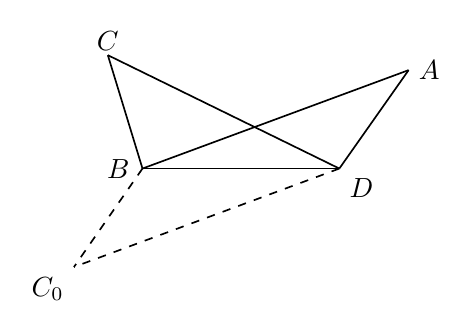
\begin{tikzpicture}[scale=1.0, semithick, every node/.style={inner sep=1.4pt}]
  \coordinate (B) at (1.30,1.40);
  \coordinate (D) at (3.80,1.40);
  \coordinate (A) at (4.68,2.65);
  \coordinate (C0) at (0.43,0.15);
  \coordinate (C) at (0.86,2.84);

  % 折起后可见的棱
  \draw (A) -- (B);
  \draw (A) -- (D);
  \draw (B) -- (D);
  \draw (B) -- (C);
  \draw (D) -- (C);

  % 折起前 C0 所在的原位置
  \draw[dashed] (B) -- (C0);
  \draw[dashed] (D) -- (C0);

  \node[right=2pt] at (A) {$A$};
  \node[left=3pt] at (B) {$B$};
  \node[below right=2pt] at (D) {$D$};
  \node[below left=2pt] at (C0) {$C_0$};
  \node[above] at (C) {$C$};
\end{tikzpicture}
